
%%%%%%%%%%%%%%%%%%%%%%% file typeinst.tex %%%%%%%%%%%%%%%%%%%%%%%%%
%
% This is the LaTeX source for the instructions to authors using
% the LaTeX document class 'llncs.cls' for contributions to
% the Lecture Notes in Computer Sciences series.
% http://www.springer.com/lncs       Springer Heidelberg 2006/05/04
%
% It may be used as a template for your own input - copy it
% to a new file with a new name and use it as the basis
% for your article.
%
% NB: the document class 'llncs' has its own and detailed documentation, see
% ftp://ftp.springer.de/data/pubftp/pub/tex/latex/llncs/latex2e/llncsdoc.pdf
%
%%%%%%%%%%%%%%%%%%%%%%%%%%%%%%%%%%%%%%%%%%%%%%%%%%%%%%%%%%%%%%%%%%%


\documentclass[runningheads,a4paper]{llncs}

\usepackage{amssymb}
\setcounter{tocdepth}{3}
\usepackage{graphicx}
\usepackage{listings}
\usepackage{xcolor} 
 
\usepackage{url}
\urldef{\mailsa}\path|shengyushen@icloud.com|    
\newcommand{\keywords}[1]{\par\addvspace\baselineskip
\noindent\keywordname\enspace\ignorespaces#1}

\begin{document}

\lstset{numbers=left, 
numberstyle= \tiny, 
keywordstyle= \color{ blue!70},commentstyle=\color{red!50!green!50!blue!50}, 
frame=shadowbox, 
rulesepcolor= \color{ red!20!green!20!blue!20} 
} 


\mainmatter  % start of an individual contribution

% first the title is needed
\title{Designing, Testing and Formally Proving a Ternary Tree Flattening Algorithm}

% a short form should be given in case it is too long for the running head
\titlerunning{Lecture Notes in Computer Science: Authors' Instructions}

% the name(s) of the author(s) follow(s) next
%
% NB: Chinese authors should write their first names(s) in front of
% their surnames. This ensures that the names appear correctly in
% the running heads and the author index.
%
\author{ShengYu Shen%
}
%
\authorrunning{Lecture Notes in Computer Science: Authors' Instructions}
% (feature abused for this document to repeat the title also on left hand pages)

% the affiliations are given next; don't give your e-mail address
% unless you accept that it will be published
\institute{
\mailsa\\
}

%
% NB: a more complex sample for affiliations and the mapping to the
% corresponding authors can be found in the file "llncs.dem"
% (search for the string "\mainmatter" where a contribution starts).
% "llncs.dem" accompanies the document class "llncs.cls".
%

\toctitle{Lecture Notes in Computer Science}
\tocauthor{Authors' Instructions}
\maketitle


\begin{abstract}
This paper describes my effort on designing, 
testing and formally proving a ternary tree flatten algorithm.
I first propose a language to describe ternary tree,
and design a scanner and a parser to analyze this language
and construct corresponding data structure in memory.
I then describe my implementation of ternary tree flatten algorithm in C,
together with a close loop testing framework that continuously generating tree
flattening it and verifying the correctness of its result.
Furthermore,
I also propose a generator mode for my program that can write out 
large tree description file.
Finally,
I formally verify this algorithm with Coq theorem prover.
\keywords{ternary tree; flattening; formal verification}
\end{abstract}


\section{Introduction}

I first define  a language to describe ternary tree in Section \ref{sec_lang}.
And then the ternary tree flatten algorithm is presented in Section \ref{sec_imp}.
After that I will show how to test this algorithm in Section \ref{sec_test}.
Finally,
I will present how to formally prove the correctness of this algorithm in 
Section \ref{sec_proof}.

In the tgz package,
t3.c contains the implementation of flatten algorithm,
while ssy.v is the Coq\cite{coq} proof of this algorithm.
Just run "make" to generate the t3.exe program.
And running it without any parameter can show you its usage.

Enjoy it.

\section{A language describing ternary tree}\label{sec_lang}

We propose a language to facilitate the job of describing ternary tree.
Its syntax is shown below in yacc\cite{yacc} format:

\begin{lstlisting}
tree :
  T0
  | ( TN tree data tree data tree )
;
data :
  D0 
  | ( DN [0-9]+ )
;
\end{lstlisting}

In this code segment,
T0 and D0 respectively mean an empty TreeNode and an empty DataNode,
while ( TN tree data tree data tree ) means a TreeNode with subtrees,
and ( DN [0-9]+ ) means a DataNode with associated \emph{value}.

So the ternary tree shown in Fig. \ref{fig_tree3} is described with the following code segment:

\begin{lstlisting}
(TN
  (TN T0 (DN 1) T0 (DN 2) T0)
  (DN 3)
  (TN
    (TN T0 (DN 4) T0 D0 T0)
    (DN 5)
    T0
    (DN 6)
    (TN T0 (DN 7) T0 D0 T0)
  )
  (DN 8)
  (TN T0 (DN 9) T0 D0 T0)
)
\end{lstlisting}


\section{Ternary tree flatten algorithm}\label{sec_imp}

\subsection{Problem definition}

A ternary tree is an extension of a binary tree, where instead of a left
and a right sub-tree pointer and a data value with value between the left
and the right subtree, there are left, center and right subtree pointers,
with two data values, one between the left and the center subtree, and one
between the center and the right subtree.

Your task is to flatten a ternary tree into an array in a depth-first
manner.
Such a tree is shown in Fig.\ref{fig_tree3}:

\begin{figure}
\centering
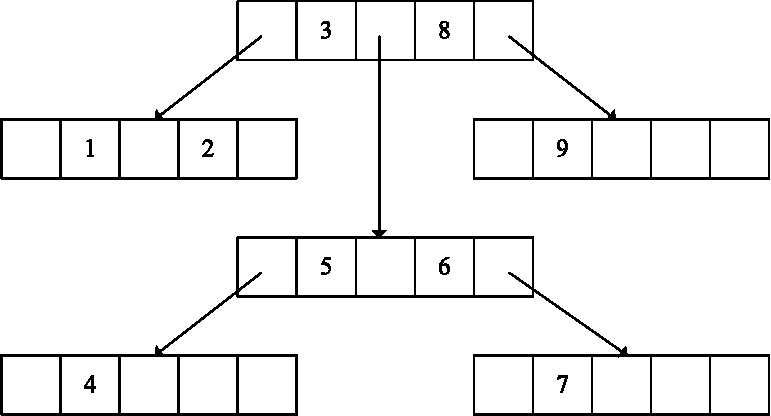
\includegraphics[width=9.2cm]{fig_tree3}
\caption{Example of ternary tree}
\label{fig_tree3}
\end{figure}

In this case, the output array should come out as follows:

1 2 3 4 5 6 7 8 9

Note that some of the values and subtrees may not be present, and this is
represented by a NULL pointer.  In this case, they should not be traversed
or be included in the output.

The data type definitions appear below:

\begin{lstlisting}
/* Define the data type */
typedef unsigned int value_t;
/* Data structures used to define the tree. */
typedef struct DataNode {
	value_t value;
} DataNode;

typedef struct TreeNode {
	struct TreeNode *left_tree;
	struct TreeNode *mid_tree;
	struct TreeNode *right_tree;
	struct DataNode *left_data;
	struct DataNode *right_data;
} TreeNode;

/* The interface to the function
flatten() that you're required to
 * implement is as follows: */
value_t * flatten (TreeNode * n, size_t * num_elements) ;
\end{lstlisting}

In this function:
"TreeNode *n" is the pointer to the root node of the tree.
"size\_t \*num\_elements" should be filled with the number of elements in
the array on exit from the function.
The return value "value\_t *" should be a pointer to an array of elements
containing the values of the flattened tree.

It is acceptable to solve this problem in either C or C++.
Please describe any assumptions you've made, and the approach you've
used to test your implementation.


\subsection{The flatten algorithm}

This algorithm is in the t3.c in the tgz package.

As shown intuitively in Fig. \ref{fig_flatten},
at each \emph{TreeNode},
my algorithm will recursively visit the three subtrees,
and collect back their array of \emph{value} items,
and merge them together with its own two \emph{value} items to form a new array,
which will finally be returned to its caller.

\begin{figure}
\centering
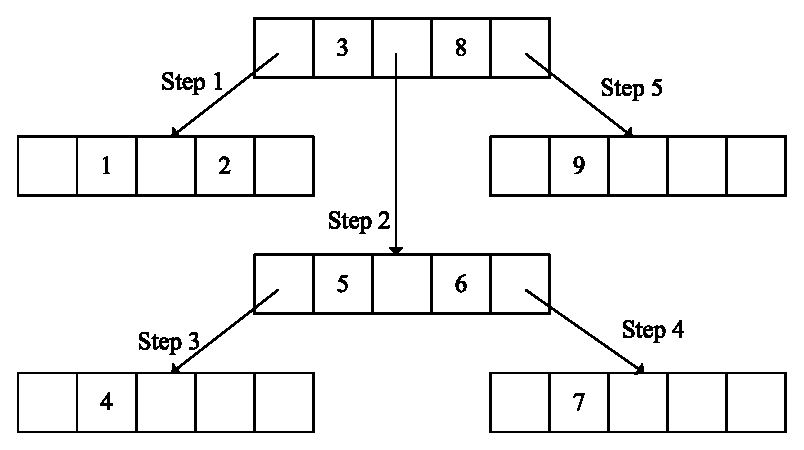
\includegraphics[width=9.2cm]{fig_flatten}
\caption{Steps in recursively enumerate a ternary tree}
\label{fig_flatten}
\end{figure}


The code that implement this idea is show below with embedded comments that explain my idea.

\begin{lstlisting}
// copying a list of data from src to dst
// the size is num
void copyData (value_t *src, value_t *dst, size_t num) {
  assert (num>=0);
  int i;
  for(i=0;i<num;i++) {
    dst[i]=src[i];
  }
  return ;
}

value_t *flatten(TreeNode *n, size_t *num_elements) 
{
  //do nothing for an empty tree
  if(n==(TreeNode*)NULL) {
    *num_elements=0;
    return (value_t*)NULL;
  } else {
    //recursively enumerate the three subtrees 
    //and get their list of data
    size_t leftSize;
    value_t *leftTreeArray=flatten(n->left_tree,&leftSize);
    size_t midSize;
    value_t *midTreeArray=flatten(n->mid_tree,&midSize);
    size_t rightSize;
    value_t *rightTreeArray=flatten(n->right_tree,&rightSize);

    size_t leftDataSize;
    if(n->left_data) {
      leftDataSize = 1;
    } else {
      leftDataSize = 0;
    }

    size_t rightDataSize;
    if(n->right_data) {
      rightDataSize = 1;
    } else {
      rightDataSize = 0;
    }

    //the total size of new array
    size_t allsize = leftSize + rightSize + 
    midSize + leftDataSize + rightDataSize;
    *num_elements = allsize;

    value_t *newArray = malloc(allsize*(sizeof(value_t)));
    //copying the left tree
    copyData(leftTreeArray,newArray,leftSize);
    size_t newindex =leftSize;

    //copying the left data and manipulate the new index
    if(leftDataSize==1) {
      newArray[newindex]=(n->left_data)->value;
      newindex ++;
    }

    //copying the mid tree
    copyData(midTreeArray,newArray+newindex,midSize);
    newindex = newindex + midSize;

    //copying the right data
    if(rightDataSize ==1) {
      newArray[newindex]=(n->right_data)->value;
      newindex ++;
    }

    //copying the right tree
    copyData(rightTreeArray,newArray+newindex,rightSize);
    
    //free all mem alloced in flattening sub tree
    free(leftTreeArray);
    free(midTreeArray);
    free(rightTreeArray);

    return newArray;
  }
}
\end{lstlisting}

\section{Testing}\label{sec_test}

\subsection{Generating ternary tree automatically}
Our tool \emph{t3} have an additional mode that generate a large tree by:


\begin{lstlisting}
Shell Prompt > t3 -gen <max depth> <density> > tree.txt
\end{lstlisting}

Here,
$<$max depth$>$ means the maximal depth of the generated tree,
while $<$density$>$ means the probability of generating a non-empty TreeNode or DataNode
at each branch.

Of course,
the user can also manually write a file according to the 
syntax described in Section \ref{sec_lang}.

We can flatten a ternary tree described in a particular file 
by running the following command in shell:
\begin{lstlisting}
Shell Prompt > t3 <tree file name>
\end{lstlisting}

\subsection{Close-loop testing framework}

As shown intuitively in Fig. \ref{fig_closeloop},
my close-loop testing framework will continuously generate a ternary tree,
put the list of \emph{value} item been inserted in this tree into a list.



\begin{figure}
\centering
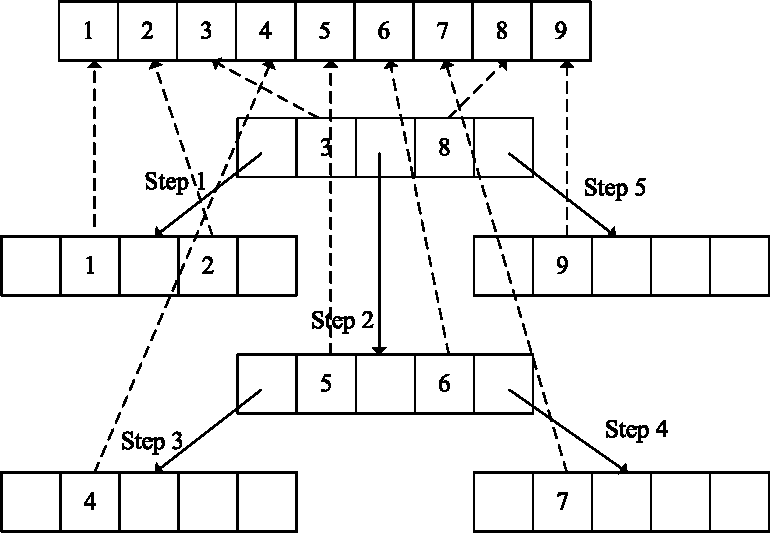
\includegraphics[width=9.2cm]{fig_closeloop}
\caption{Generating ternary tree with all its \emph{value} item inserted into a list}
\label{fig_closeloop}
\end{figure}

As shown in Fig. \ref{fig_closeloop2},
After the flattening algorithm flattens the ternary tree,
it can compare the resulting array with the list to confirm its result is correct.

\begin{figure}
\centering
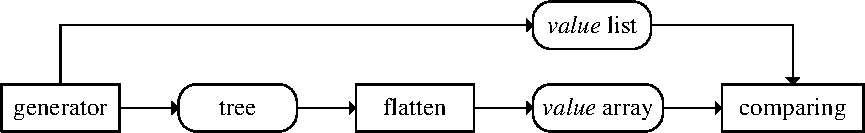
\includegraphics[width=9.2cm]{fig_closeloop2}
\caption{Flattening a ternary tree and comparing the \emph{value} array}
\label{fig_closeloop2}
\end{figure}


This framework is called by running the following command in shell:

\begin{lstlisting}
Shell Prompt > t3 -l
\end{lstlisting}


This framework will continuously increase the depth of the generated tree from 10,
and run forever.
The density for each generated tree is randomly determined before each iteration.



\section{Formal proof of the flatten algorithm}\label{sec_proof}

This proof is in the ssy.v file in the tgz package.
\subsection{subsecdef}
I use the coq theorem prover\cite{coq} to prove the correctness of this algorithm.
I will explain the proof step by step.

I first invoke all the related Coq library:

\begin{lstlisting}
Require Import Arith.
Require Import List.
Require Import Bool.
Import ListNotations.
Open Scope nat_scope.
Open Scope list_scope.
\end{lstlisting}

I then define the two data structure DataNode and TreeNode:

\begin{lstlisting}
(*definition of the two data structure of tenary tree*)
Inductive DataNode : Set :=
D0
| DN : nat -> DataNode.

Inductive TreeNode : Set :=
T0 : TreeNode
| TN : TreeNode->DataNode->TreeNode->
DataNode->TreeNode->TreeNode.
\end{lstlisting}

Then I define how to flatten a DataNode:

\begin{lstlisting}
(*flattening the DataNode*)
Definition flatten_DataNode :=
fun dn:DataNode =>
  match dn with
  D0 => nil
  | DN n => cons n nil 
  end.
\end{lstlisting}

I further define how to flatten a TreeNode,
this is exactly the algorithm defined in Section\ref{sec_imp}:

\begin{lstlisting}
(*flattening the TreeNode*)
Fixpoint  flatten (tn:TreeNode) : list nat :=
  match tn with
  T0 => nil
  | TN lefttree leftdata midtree rightdata righttree => 
    let leftlist :=flatten lefttree in
    let midlist  :=flatten midtree in
    let rightlist:=flatten righttree in
    let leftdatalist := flatten_DataNode leftdata in
    let rightdatalist:= flatten_DataNode rightdata in
    leftlist++leftdatalist++midlist++
    rightdatalist++rightlist
  end.
\end{lstlisting}

At this point,
you can take test this reformulated version on ternary tree by running:

\begin{lstlisting}
Eval compute in flatten <tree>.
\end{lstlisting}

For example:

\begin{lstlisting}
(*test drive on the flatten algorithm*)
Eval compute in flatten (TN T0 D0 T0 (DN 1) T0).
Eval compute in flatten 
(TN
  (TN T0 (DN 1) T0 (DN 2) T0)
  (DN 3)
  (TN
    (TN T0 (DN 4) T0 D0 T0)
    (DN 5)
    T0
    (DN 6)
    (TN T0 (DN 7) T0 D0 T0)
  )
  (DN 8)
  (TN T0 (DN 9) T0 D0 T0)
).
\end{lstlisting}

I then define predicate stating that a value $n$ appear in a DataNode $dn$:

\begin{lstlisting}
(*a predicate meaning that n is in dn*)
Definition inDN (n:nat) (dn:DataNode) :Prop :=
  match dn with
  D0 => False
  | DN v => v=n
  end.
\end{lstlisting}

Similarly,
I define a predicate stating that a value $n$ appear in a TreeNode $tn$:

\begin{lstlisting}
Fixpoint inTN (n:nat) (tn:TreeNode) :Prop :=
  match tn with
  T0 => False
  | TN lefttree leftdata midtree rightdata righttree =>
    (inTN n lefttree)\/
    (inDN n leftdata)\/
    (inTN n midtree)\/
    (inDN n rightdata)\/
    (inTN n righttree)
  end.
\end{lstlisting}

\subsection{subsecproof}

Next,
I prove that the $inDN$ operator is preserved by $flatten\_DataNode$:

\begin{lstlisting}
Lemma inDN_in_flattenDataNode :
  forall (n:nat) (dn:DataNode),
    (inDN n dn) -> (In n (flatten_DataNode dn)).
Proof.
intros.
induction dn.
elim H.
elim H.
simpl.
auto.
Qed.
\end{lstlisting}

Similarly,
I prove that the $inTN$ operator is preserved by $flatten$:

\begin{lstlisting}
(*in operator is preserved by flatten
that is to say, some element in a 
TreeNode is also in its flatten result*)
Theorem in_trans_flatten :
  forall (n:nat) (tn:TreeNode),
    (inTN n tn) -> (In n (flatten tn)).
Proof.
intros.
induction tn.
auto.
simpl in *.
repeat rewrite in_app_iff .
elim H.
intros.
left.
auto.
intros.
right.
elim H0.
intros.
left.
apply inDN_in_flattenDataNode.
auto.
intros.
right.
elim H1.
intros.
left.
apply IHtn2.
auto.
intros.
right.
elim H2.
intros.
left.
apply inDN_in_flattenDataNode.
auto.

intros.
right.
apply IHtn3.
auto.
Qed.
\end{lstlisting}


Again, 
I will prove the $inDN$ operator is reversely preserved by $flatten\_DataNode$:

\begin{lstlisting}
Lemma in_flattenDataNode_inDN :
  forall (n:nat) (dn:DataNode),
    (In n (flatten_DataNode dn)) -> (inDN n dn).
Proof.
intros.
(*once again induction can expand dn on both hyp and goal
while case cab only expand goal*)
induction dn.
auto.
simpl.
elim H.
auto.
simpl.
intro.
elim H0.
Qed.
\end{lstlisting}

Similarly,
I prove the $inTN$ operator is reversely preserved by $flatten$ with some lemmas:

\begin{lstlisting}
 
Lemma in_3 :
  forall (a :nat) (l1 l2 l3: list nat),
    (In a (l1++l2++l3)) -> (In a l1)\/(In a l2)\/(In a l3).
Proof.
intros.
induction l1.
(*this is simply in all place*)
simpl  in *.
right.
apply in_app_or.
assumption.
elim H.
intros.
left.
rewrite H0.
apply in_eq.
intros.
(*very useful in using hyps IHl0 with "A-> B" and H0 with "A"*)
destruct (IHl1 H0).
left.
apply in_cons.
assumption.
right.
assumption.
Qed.

Lemma in_4 :
  forall (a :nat) (l1 l2 l3 l4: list nat),
    (In a (l1++l2++l3++l4)) -> (In a l1)\/(In a l2)\/(In a l3)\/(In a l4).
Proof.
intros.
induction l1.
simpl in *.
right.
apply in_3.
assumption.
elim H.
intros.
left.
rewrite H0.
apply in_eq.
intros.
destruct (IHl1 H0).
left.
apply in_cons.
auto.
right.
auto.
Qed.


Lemma in_5 :
  forall (a :nat) (l1 l2 l3 l4 l5: list nat),
    (In a (l1++l2++l3++l4++l5)) -> (In a l1)\/(In a l2)\/(In a l3)\/(In a l4)\/(In a l5).
Proof.
intros.
induction l1.
simpl in *.
right.
apply in_4.
auto.
elim H.
intros.
left.
rewrite H0.
apply in_eq.
intros.
destruct (IHl1 H0).
left.
apply in_cons.
auto.
right.
auto.
Qed.

Theorem in_trans_flatten_rev :
  forall (n:nat) (tn:TreeNode),
    (In n (flatten tn)) -> (inTN n tn).
Proof.
intros.
induction tn.
auto.
simpl in *.
destruct ((in_5 n (flatten tn1) (flatten_DataNode d) (flatten tn2) (flatten_DataNode d0) (flatten tn3)  )H).
left.
apply IHtn1.
auto.
right.
(*another powerful trick that break A \/B\/... into A and B\/...*)
induction H0.
left.
apply in_flattenDataNode_inDN .
auto.
elim H0.
intros.
right.
left.
apply IHtn2.
auto.
intro.
right.
right.
elim H1.
intros.
left.
apply in_flattenDataNode_inDN .
auto.
intros.
right.
apply IHtn3.
auto.
Qed.

\end{lstlisting}


With Theorems $in\_trans\_flatten$ and $in\_trans\_flatten\_rev$ presented above,
we can be sure that $flatten$ algorithm does not change the set of $value$.



\section{REFERENCES}

\begin{thebibliography}{10}
\bibitem{yacc}
 Johnson, Stephen C. (1975). 
 "Yacc: Yet Another Compiler-Compiler". AT\&T Bell Laboratories Technical Reports 
 (AT\&T Bell Laboratories Murray Hill, New Jersey 07974) (32).
\bibitem{coq}
Yves Bertot, Pierre Castéran , ``Interactive Theorem Proving and Program Development
Coq’Art: The Calculus of Inductive Constructions,'' 
in Texts in Theoretical Computer Science An EATCS Series,Springer 2004. 
\end{thebibliography}

\end{document}
